\chapter{Entwicklung der Gleisfreimeldeanlage}\label{text:Entwicklung-der-GFA}

In den vorangegangen Kapiteln wurde beschrieben, wie die Stellwerkstechnik bei realen Eisenbahnen funktioniert und mögliche Umsetzungen für die Automatisierung einer Modelleisenbahn vorgestellt. In diesem Kapitel soll die Entwicklung der Gleisfreimeldeanlage beschrieben werden.

\input{Text/4-Entwicklung-der-GFA/Achszähler.tex}
\newpage
\section{Gleisfreimeldung}\label{text:Grundlagen:Gleisfreimeldung}

Die Gleisfreimeldung ist ein wichtiges Element der Sicherungstechnik im Schienenverkehr. Ihre scheinbar einfache Aufgabe ist es, das Frei- oder Besetztsein eines Gleisabschnittes zu überwachen und dem Stellwerk zu melden. Heutzutage sind zwei verschiedene Arten der Gleisfreimeldung im Einsatz: Gleisstromkreise und Achszähler. In diesem Abschnitt werden nach einer Betrachtung der Historie, beide Systeme vorgestellt und ihre Funktionsweise erläutert.

\subsection{Historische Gleisfreimeldung}\label{text:Grundlagen:Gleisfreimeldung:Historische-Gleisfreimeldung}

\subsection{Gleisstromkreis}\label{text:Grundlagen:Gleisfreimeldung:Gleisstromkreis}

Gleisstromkreise bestimmen den Belegungszustand eines Freimeldeabschnitts über Stromkreise, die durch die Räder der Schienenfahrzeuge geschlossen werden.~\cite[][S. 47]{bib:Sicherung-des-Schienenverkehrs} \autoref{abb:Grundlagen:Gleisfreimeldung:Gleisstromkreis} zeigt den Aufbau eines Gleisstromkreises.

\begin{figure}[H]
    \centering
    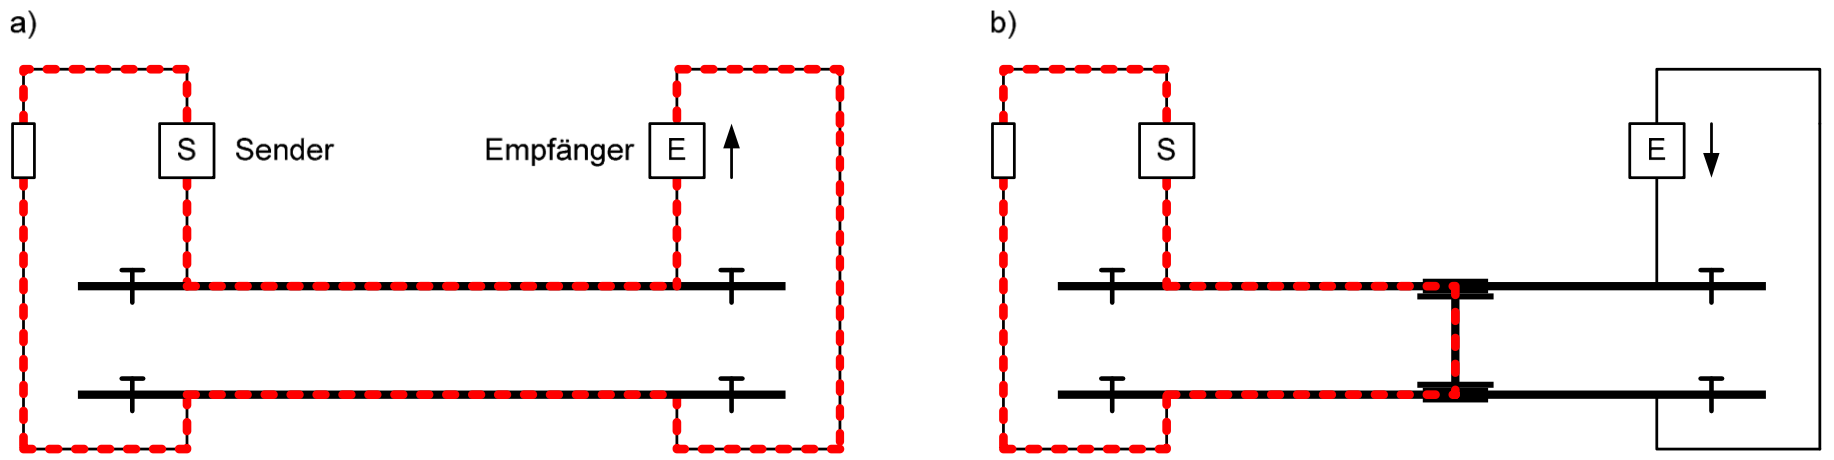
\includegraphics[width=0.7\textwidth]{Assets/Images/2-Grundlagen/Gleisstromkreis.png}
    \caption{Aufbau eines Gleisstromkreises~\cite[][S. 47]{bib:Sicherung-des-Schienenverkehrs}}\label{abb:Grundlagen:Gleisfreimeldung:Gleisstromkreis}
\end{figure}

\textquote{Gleisstromkreise arbeiten nach dem Ruhestromprinzip. Dabei liegt in Grundstellung (freies Gleis) ein geschlossener Stromkreis vor.}~\cite[][S. 47]{bib:Sicherung-des-Schienenverkehrs} Wird ein Gleisabschnitt durch ein Schienenfahrzeug belegt, wird der Stromkreis unterbrochen. Die Unterbrechung des Stromkreises wird vom Stellwerk registriert und als belegt gemeldet.~\cite[][S. 47]{bib:Sicherung-des-Schienenverkehrs} Befindet sich eine Achse im Gleisfreimeldeabschnitt, so wird der Stromkreis geschlossen und der Abschnitt dem Stellwerk besetzt gemeldet.~\cite[][S. 47]{bib:Sicherung-des-Schienenverkehrs}

Ein großer Vorteil von Gleisstromkreisen ist, dass sie in der Lage sind auch stehende Fahrzeuge zu erkennen. Allerdings kann es bei Störungen der Leitfähigkeit der Schienen zu Fehlmeldungen kommen.

\subsection{Achszähler}\label{text:Grundlagen:Gleisfreimeldung:Achszähler}

Achszähler bestimmen den Belegungszustand eines Freimeldeabschnitts über die Zählung der ein- und ausfahrenden Achsen.~\cite[][S. 53]{bib:Sicherung-des-Schienenverkehrs} \autoref{abb:Grundlagen:Gleisfreimeldung:Achszaehlkreis} zeigt den Aufbau eines Achszählkreises.

\begin{figure}[H]
    \centering
    \includegraphics[width=0.7\textwidth]{Assets/Images/2-Grundlagen/Achszählkreis.png}
    \caption{Aufbau eines Achszählkreises~\cite[][S. 53]{bib:Sicherung-des-Schienenverkehrs}}\label{abb:Grundlagen:Gleisfreimeldung:Achszaehlkreis}
\end{figure}

Am Gleis sind Elektromagnete (Schienenkontakte), angebracht, deren Magnetfeld bei Überfahrt eines Rades gestört wird. Diese Störung wird registriert und die Achse gezählt. Achszähler sind in der Lage, die Fahrtrichtung zu bestimmen, indem zwei nah beieinander liegende Schienenkontakte verbaut werden.~\cite[][S. 53 ff.]{bib:Sicherung-des-Schienenverkehrs} \autoref{abb:Grundlagen:Gleisfreimeldung:Doppelter-Schienenkontakt} zeigt einen solchen doppelten Schienenkontakt.

\begin{figure}[H]
    \centering
    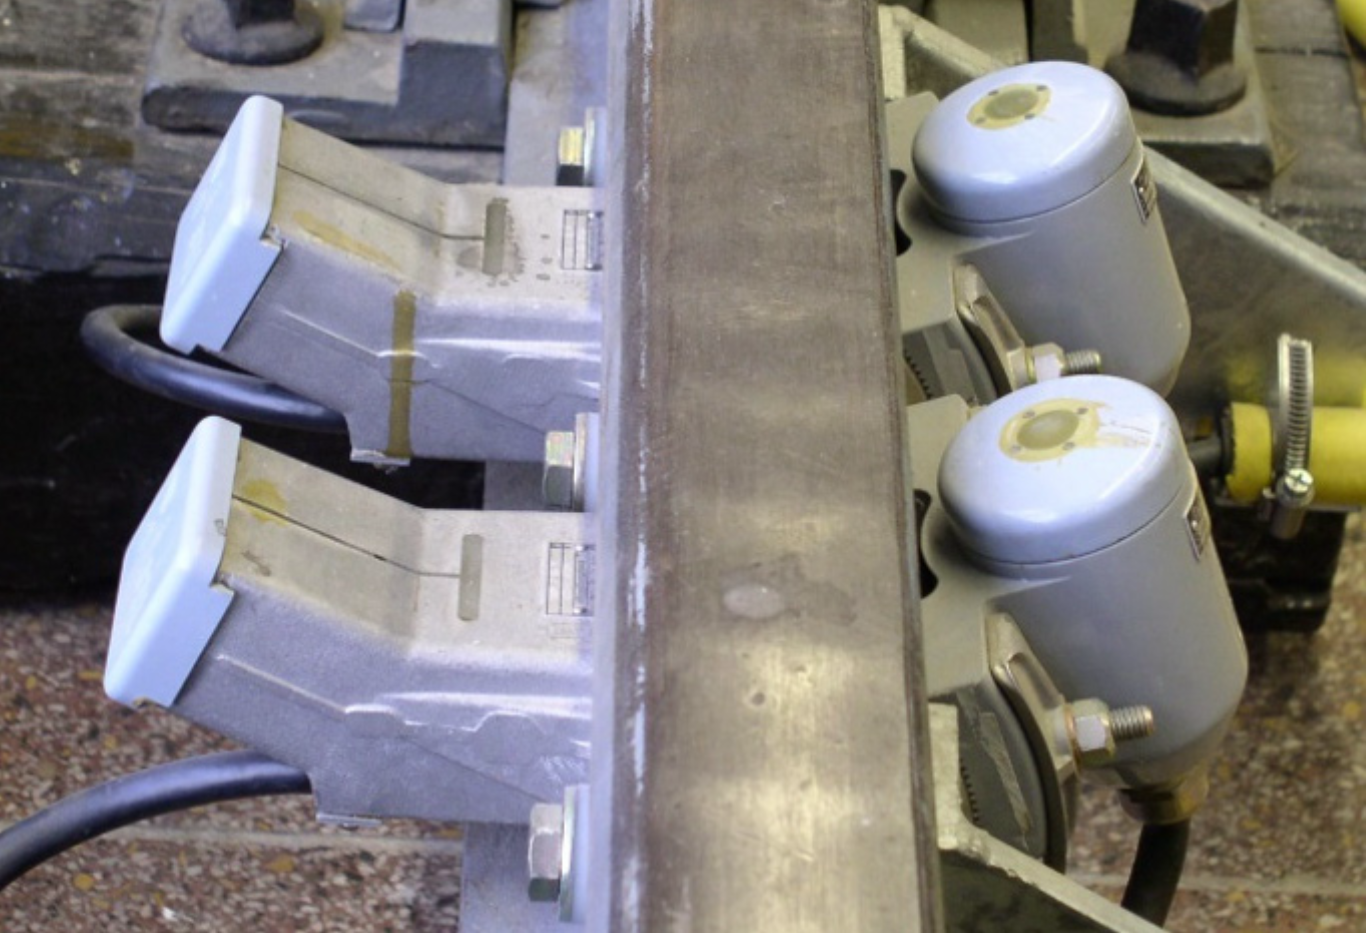
\includegraphics[width=0.7\textwidth]{Assets/Images/2-Grundlagen/Doppelter-Schienenkontakt.png}
    \caption{Doppelter Schienenkontakt~\cite[][S. 54]{bib:Sicherung-des-Schienenverkehrs}}\label{abb:Grundlagen:Gleisfreimeldung:Doppelter-Schienenkontakt}
\end{figure}

Im Gegensatz zu Gleisstromkreisen sind Achszähler nicht in der Lage stehende Fahrzeuge zu erkennen, können jedoch die Fahrtrichtung feststellen.

\newpage
\section{Softwaretests}\label{text:Entwicklung-der-GFA:Softwaretests}

Die Softwaretests sind ein wichtiger Bestandteil der Softwareentwicklung. Sie dienen dazu, die Funktionalität der Software zu überprüfen und Fehler zu finden. In diesem Abschnitt werden die Softwaretests für die Gleisfreimeldeanlage beschrieben.\newline
Die Tests für die Gleisfreimeldeanlage sind Software-seitig in zwei Kategorien unterteilt:
\begin{itemize}
    \item Tests für Geraden
    \item Tests für Weichen
\end{itemize}
Die Test-Skripte wurden nach und nach entwickelt und immer wieder ausgeführt. Somit wurden zunächst die Methoden zur Initialisierung der einzelnen Komponenten getestet und später die Methoden zur Überprüfung der Funktionalität der Gleisfreimeldeanlage.

\subsection{Tests für Geraden}\label{text:Entwicklung-der-GFA:Softwaretests:Tests-für-Geraden}

Das Testprogramm startet mit der Initialisierung der einzelnen Komponenten. Da das Skript zu lange ist um es hier komplett darzustellen, wird nur ein Ausschnitt dessen gezeigt. Für das Verständnis ist es wichtig die folgenden Definitionen zu kennen:
\begin{itemize}
    \item p1, p2, p3, p4 sind Kontaktpunkte
    \item d1 ist ein gerichteter Achszähler, der die Kontaktpunkte p1 und p2 verwendet
    \item d2 ist ein gerichteter Achszähler, der die Kontaktpunkte p3 und p4 verwendet
    \item c ist ein Counter/ Streckenabschnitt
    \item v ist die Gleisfreimeldeanlage
\end{itemize}


\newpage
\section{Hardwaretests}\label{text:Entwicklung-der-GFA:Hardwaretests}

Im Rahmen der Entwicklungsprozesse einer Gleisfreimeldeanlage kommt den Hardwaretests eine ebenso signifikante wie den Softwareprüfungen zustehende Bedeutung zu. Diese Tests dienen der Verifizierung der Funktionsfähigkeit und der Leistungsfähigkeit der physischen Komponenten unter realitätsnahen Einsatzbedingungen. Im nachfolgenden Abschnitt wird eine umfassende Darstellung der für die Sicherstellung der Zuverlässigkeit und Effizienz der Gleisfreimeldeanlage unerlässlichen Hardwaretests vorgenommen. Es werden die angewendeten Methodiken, Instrumente und Verfahrensweisen erörtert, welche essentiell sind, um die Funktionalität, Beständigkeit und die Interoperabilität der Hardwarekomponenten zu evaluieren. Dies geschieht mit dem Ziel, die Einhaltung der hohen Sicherheits- und Leistungsstandards im Eisenbahnwesen zu gewährleisten.

\subsection{Aufbau}

Die Hardwaretests der Gleisfreimeldeanlage kombinieren in erster Linie die Reed-Kontakte mit der Software und überprüfen deren Funktionalität. Um schnell verschiedene Umstände testen zu können und die Fehlersuche zu minimieren wurden diese Tests auf einem Steckbrett durchgeführt. Das Steckbrett ist in \autoref{abb:HWTest-bb} dargestellt.
\begin{figure}[H]
    \centering
    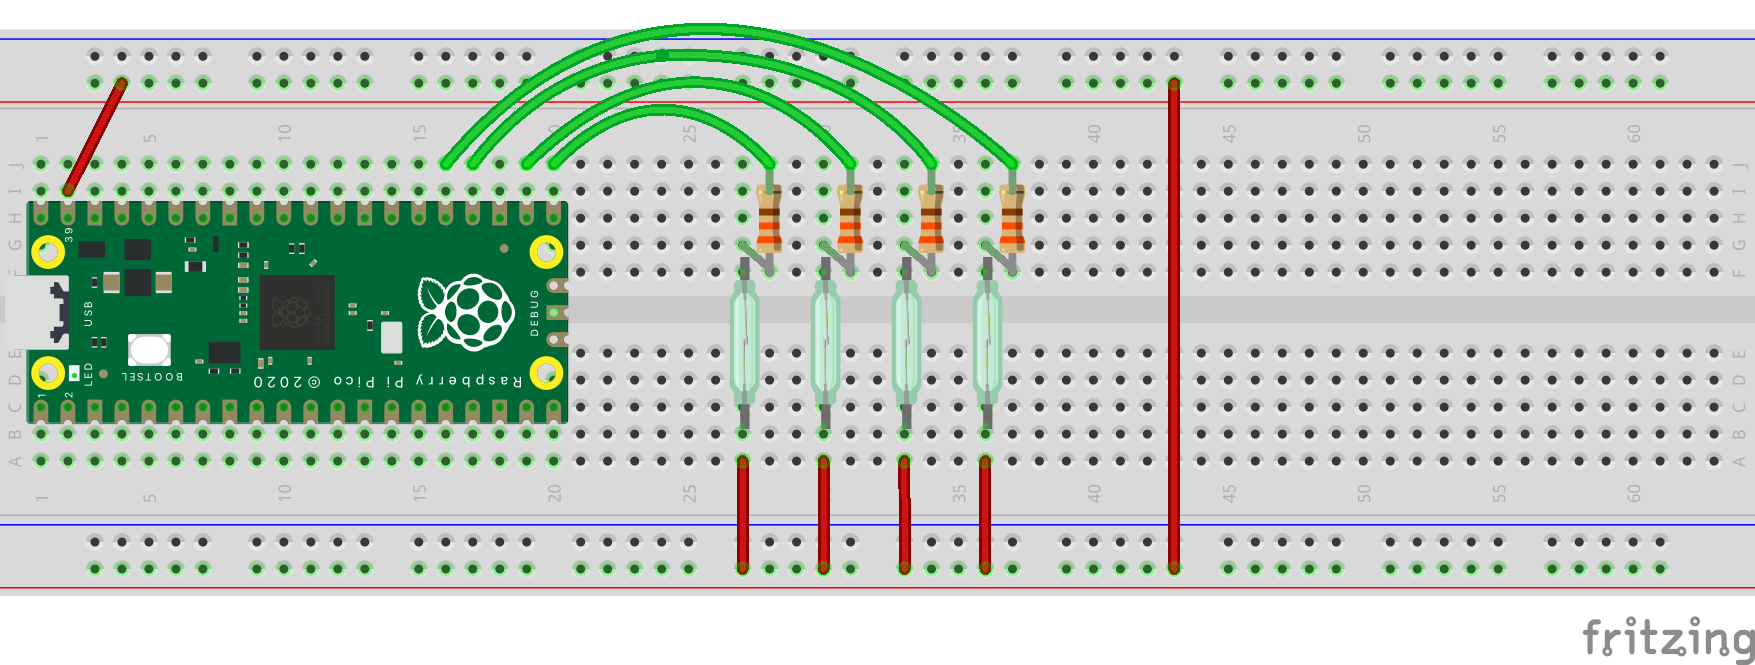
\includegraphics[width=0.7\textwidth]{Assets/Images/4-Entwicklung-der-GFA/Reed-Test_bb.png}
    \caption{Aufbau der Hardwaretests auf einem Steckbrett}\label{abb:HWTest-bb}
\end{figure}

Um die Zustände der Software zu visualisieren, wurden zusätzlich LEDs auf dem Steckbrett verbaut. Diese LEDs zeigen sowohl den aktuellen Zählerstand des simulierten Streckenabschnitts, als auch den aktuellen Error-Code in 3-Bit Darstellung an. Die Schaltung hinter den LEDs ist trivial und wird daher nicht weiter beschrieben.

\subsection{Testszenarien}

Die Testszenarien für die Hardwaretests sind in erster Linie auf die Software zurück zu führen. Hierbei verliefen die ersten Tests zunächst ungeordnet und bei Bedarf. Nach und nach wurden aber auch spezifische Testszenarien entwickelt, umd die Funktionalität der Software zu überprüfen. Diese Tests sind kausal zu den Softwaretests welche in \autoref{text:Entwicklung-der-GFA:Softwaretests:Tests-für-Geraden} \nameref{text:Entwicklung-der-GFA:Softwaretests:Tests-für-Geraden} beschrieben sind.
